\section{Durchführung}
\label{sec:Durchführung}

\subsection{Vermessung von Spulen/Magnetfeld von Spulen}

Zuerst sollen die magnetischen Flussdichten von zwei Spulen - einer kurzen mit einer Länge 
$l = 5.5\, \si{\centi\meter}$ und $n = 100\,$ Windungen, sowie einer langen Spule mit einer Länge
$l = 15.8\, \si{\cm}$ und $n = 300\,$ Windungen - gemessen werden. Dies soll mithilfe einer
(longitudinalen) Hall-Sonde verwirklicht werden, die entlang der Spulenmitte bei konstanter Spannung U und konstantem
Strom I, die magnetische Flussdichte misst. Dabei sollen von beiden Seiten Messwerte sowohl außerhalb, als auch
innerhalb der Spule aufgenommen werden.
Die dabei erhaltenen Ergebnisse sollen graphisch aufgetragen und mit dem Theoriewert des magnetischen Flusses
innerhalb der Spulen verglichen werden.

\begin{figure}[H]
    \centering
    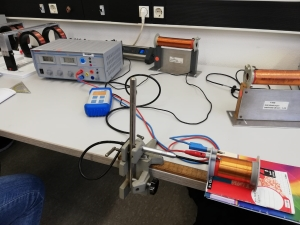
\includegraphics{Spule2.jpg}
    \caption{Versuchsaufbau zur Vermessung einer kurzen Spule }
    \label{KurzeSpule}
    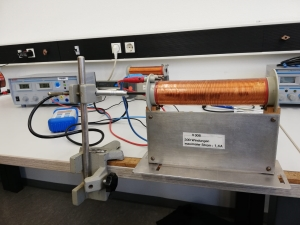
\includegraphics{Spule1.jpg}
    \caption{Versuchsaufbau zur Vermessung einer langen Spule }
    \label{LangeSpule}
\end{figure}


\subsection{Vermessung von Helmholtzspulen/Magnetfeld eines Spulenpaares}

In diesem Teil soll die magnetische Flussdichte B von einem Helmholtzspulenpaar untersucht werden.
Dazu werden zwei identische Spulen, mit Radius $r = 12.5\, \si{\cm}$, Breite $b = 3.3\, \si{\centi\meter}$, die
jeweils $n = 100$ Windungen besitzen, in drei unterschiedlichen Abständen voneinander platziert. Dabei ist zu beachten,
dass die Spulen ohne einen seitlichen Versatz und ohne Drehwinkel zueinander angeordnet sein müssen.
Die notierten Werte geben den Abstand von dem Mittelpunkt der einen Spule zum Mittelpunkt der anderen Spule an. 
Auch hier gilt es das magnetische Feld auf einer Achse, die durch die Spulenmitten verläuft, bei konstanter
Stromstärke I, sowie konstanter Spannung U zu messen. Es sollen sowohl Messwerte zwischen den Spulen, als auch 
außerhalb der Spulen, mithilfe einer (transversalen) Hallsonde aufgenommen werden. Die aufgeschriebenen 
Werte beziehen sich auf den Abstand von dem nach innen gerichteten Rand einer Spule zur Hallsonde.
Die so ermittelten Werte sollen graphisch dargestellt und mit den Theoriewerten verglichen werden.

\begin{figure}[H]
    \centering
    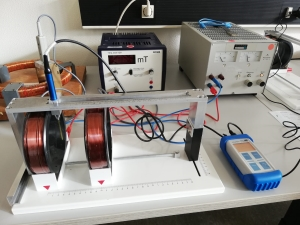
\includegraphics{Helmholtzspule.jpg}
    \caption{Versuchsaufbau zur Vermessung von Helmholtzspulen}
    \label{Helmholtzspulen}
\end{figure}

\subsection{Hysteresekurve}

Zuletzt soll die Hysteresekurve einer Ringspule mit $n = 595\,$ Windungen, einem Luftspalt der 
Breite $b = 3\, \si{\milli\meter}$ und einem Durchmesser von $d = 26\, \si{\centi\meter}$ aufgezeichnet werden. Dazu
soll der Spulenstrom zunächst von $I = 0\, \si{\ampere}$ in zehn Schritten auf $I = 0\, \si{\ampere}$ hochgestellt werden 
und anschließend ebenfalls in zehn Schritten wiederum auf $I = 0\, \si{\ampere}$ herabgesetzt werden. Nach einer Umpolung 
wird der eben beschriebene Vorgang wiederholt. Wenn dies abgeschlossen ist, soll nach einer weiteren Umpolung die Stromstärke
ein letztes Mal von $I = 0\, \si{\ampere}$ in zehn Schritten auf $I = 10\, \si{\ampere}$ hochgeregelt werden. Die 
Messwerte für die magnetische Flussdichte werden mit einer transversalen Hallsonde aufgenommen. Die Ergebnisse sollen 
graphisch dargestellt werden und zusätzlich sollen Sättiungsmagnetisierung $U_S$, Remanenz $U_r$ und 
Koerzitivkraft $H_c$ ermittelt werden.

\begin{figure}[H]
    \centering
    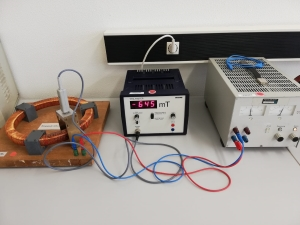
\includegraphics{Ringspule.jpg}
    \caption{Versuchsaufbau zur Ermittlung der Hysteresekurve}
    \label{Ringspule}
\end{figure}